\section{SOTA}

%%%%%%%%%%%%%%%%%%%%%%%%%%%%%%%%%%%%%%%%%
%              MiDas
%%%%%%%%%%%%%%%%%%%%%%%%%%%%%%%%%%%%%%%%%
All the methods introduced suffer from poor generalization and poor transferability to other datasets and to unconstrained scenes.
In fact the main depth estimation datasets are not sufficiently rich to train a robust model.
The advancement that makes a leap forward is MiDas \cite{MiDas}, which stands for "Mixing Datasets".
MiDas is a technique for training a depth estimation model on diverse labeled data by using a loss function that is invariant to the various differences among datasets.
The authors of \cite{MiDas} also used 3D-movies as source of stereo data and they did a great work in cleaning it up and converting it to suitable disparity maps.
Three main incompatibilities arise across different datasets:
\begin{enumerate}
	\item Ground truth representation, which can be a depth map or a disparity map
	\item Scale ambiguity, some datasets use relative depth and others provide up-to-scale depth maps
	\item Shift ambiguity, in particular in 3D movies stereo pairs present a global disparity shift.
\end{enumerate}
First: they choose to work in disparity space.
Then, when comparing a ground truth disparity map $\mathbf{d}_{gt}$ and a predicted disparity map $\mathbf{d}_{pred}$ they scale and shift the two so that they have zero shift and unit scale.
They approximate the idea of "scale" and "shift" by means of two functions $s$ and $t$:
\[
	t(\mathbf{d}) := \mathop{\text{median}}_{p \in \mathbf{d}}(\mathbf{d}(p))
\] \[
	s(\mathbf{d}) := \mathop{\text{mean}}_{p \in \mathbf{d}} \big| \mathbf{d}(p) - t(\mathbf{d}) \big|
\] \[
	\hat{\mathbf{d}}_{pred} = \frac{\mathbf{d}_{pred} - t(\mathbf{d}_{pred})}{s(\mathbf{d}_{pred})}
\] \[
	\hat{\mathbf{d}}_{gt} = \frac{\mathbf{d}_{gt} - t(\mathbf{d}_{gt})}{s(\mathbf{d}_{gt})}
\]
Finally their scale and shift invariant($ssi$) loss is:
\[
	\mathcal{L}_{ssi} = \mathop{\text{mean}}_{p \in \mathbf{d}} \big| \hat{\mathbf{d}}_{pred}(p) - \hat{\mathbf{d}}_{gt}(p)\big|
\]
They regularize it using the following term, which biases the prediction discontinuities to match the ones in the respective ground truth:
\[
	\mathcal{L}_{reg} = \mathop{\text{mean}}_{p \in \mathbf{d}}
		\left(
			\big| \partial_{x} (\hat{\mathbf{d}}_{pred} - \hat{\mathbf{d}}_{gt}) \big| +
			\big| \partial_{y} (\hat{\mathbf{d}}_{pred} - \hat{\mathbf{d}}_{gt}) \big| 
		\right)(p)
\]
Lastly they discuss the mixing strategies for sampling the datasets in the mini-batches of the stochastic gradient descent algorithm.
They propose to use a Pareto-optimal strategy from \cite{pareto}, this mixing-strategy will be used in many subsequent works while the loss they introduced is often replaced by the scale-invariant loss from \cite{Eigen}.
They use some datasets for training and some for testing, using the experimental protocol called \textit{zero-shot cross-dataset transfer}.
The model architecture is an encoder-decoder-like model as in \cite{ReDWeb}. Their full work and code can be found at \url{https://github.com/isl-org/MiDaS}, here the matter has been simplified for brevity.

%%%%%%%%%%%%%%%%%%%%%%%%%%%%%%%%%%%%%%%%%
%              PatchFusion
%%%%%%%%%%%%%%%%%%%%%%%%%%%%%%%%%%%%%%%%%
Li et al. \cite{PatchFusion} address the problem of metric monocular depth estimation for high-resolution inputs.
Their method, PatchFusion, aligns with so called \textit{Tile-Based Methods}.

% architecture
\begin{figure}
	\centering
	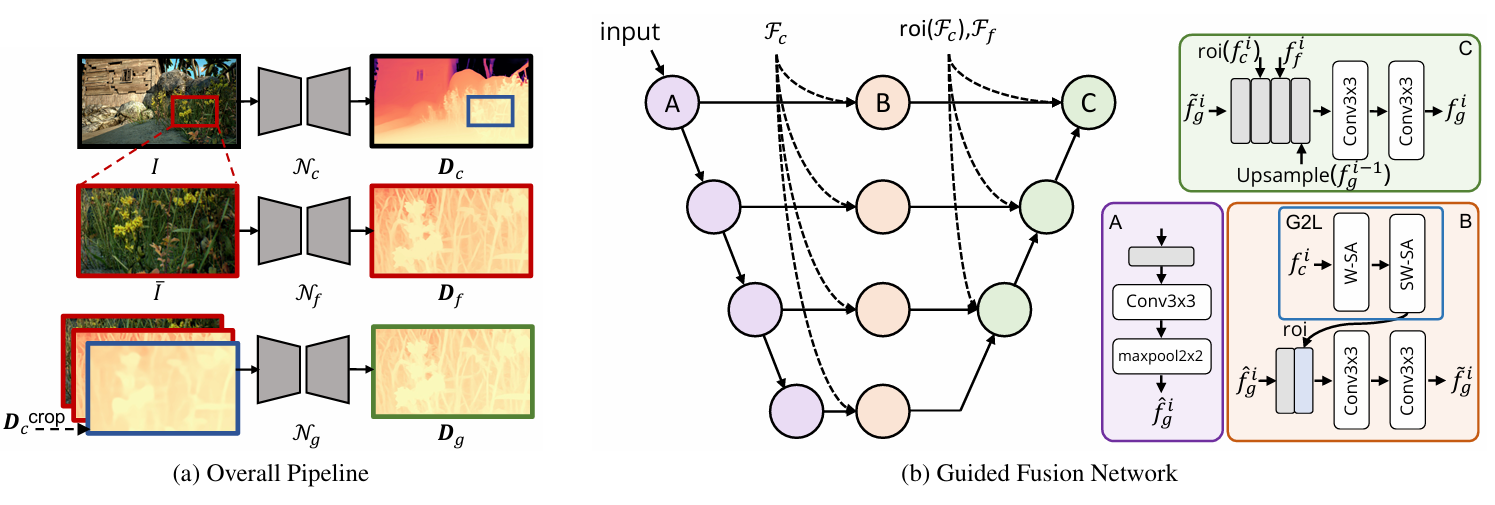
\includegraphics[scale=0.3]{figs/patchfusion}
	\caption{Li et al. architecture \cite{PatchFusion}. \label{fig:patchfusion}}
\end{figure}

The architecture employed is composed of three networks: a global-scale aware prediction network which takes as input a high-resolution down-sampled image and outputs a coarse depth map; a patch-wise depth prediction network which takes as input an image patch and outputs its fine relative depth map; a guided-fusion network.
The guided-fusion network is intricate, but its role is to further process the fine depth map of a patch to make it scale-aware.
It takes as inputs the fine depth map and the corresponding patches in the original image and in the coarse depth map.
With this machinery is now possible to divide a high-resolution image in patches and compute a depth map for each patch, obtaining a depth map for the whole image, but patch artifacts are yet to be removed.
To this end \textit{Consistency-Aware Training} is performed by subdividing the images in overlapping patches and minimizing also the agreement between the patch depth maps and feature maps.
If $\rho_{1}$ and $\rho_{2}$ are two overlapping patch depth maps and $\phi_{1}$, $\phi_{2}$ their respective feature maps, the consistency-aware loss term is:
\[
	\mathcal{L}_{consistency} = \mathop{\text{mean}}_{p \in \phi_{1} \cap \phi_{2}} \left( \big\| \phi_{1}(p) - \phi_{2}(p) \big\|_{2} + \mu \big| \rho_{1}(p) - \rho_{2}(p) \big| \right)
\]
Where $\mu$ is, with no surprises, a hyperparameter.
One important technical detail of their guided-fusion network is that SwinTransformer layers \cite{swin} are used to process feature maps and preserve global context \cite{PatchFusion}.
Code and everything at \url{https://zhyever.github.io/patchfusion/}.\\
\\
Ke et al. \cite{Marigold} prove that a comprehensive representation of the visual world is the cornerstone of (relative) monocular depth estimation.
Their insight is to use priors learned by generative diffusion models to enable more generalizable depth estimation, in particular they adopt Stable Diffusion v2 \cite{StableDiffusionV2} pretrained Variational Auto Encoder(VAE) and Latent Diffusion U-Net.
Monocular depth estimation is here posed as a conditional denoising diffusion generation task.
The idea is to teach a model called "diffusion model" to clean a depth map from noise conditioned to the corresponding RGB image.
More formally consider an RGB image $I$, its depth map $\rho$ and its noise corrupted depth map $\tilde{\rho}_{0}$ (which can be so corrupted to be just sampled random noise, i.e. $\rho$ needn't be known), the diffusion model takes as input the two and outputs a less noisy depth map $\tilde{\rho}_{1}$.
The noise is modeled as additive, hence $\tilde{\rho}_{1} = \tilde{\rho}_{0} + \epsilon(I, \tilde{\rho}_{0})$, where $\epsilon$ is the computed noise to remove.
After repeating the procedure a few times the resulting depth map is expected to match the ground truth depth map: $\tilde{\rho}_{T} \approx \rho$.
Actually, all this process takes place in a \textit{latent space}, meaning that instead of working with depth maps and images, the diffusion model works with their lower dimensional representations computed by the encoder $\mathcal{E}$ from the pretrained Stable Diffusion VAE(and with fixed parameters) and noise is added in that space.
For getting the final depth estimate the decoder $\mathcal{D}$ from the same VAE is used.
I'm not giving all the details here, but one thing to know is how a pretrained model that works with RGB images can work with depth maps: depth maps are first affinely trasformed to be in approximately the range $[-1, +1]$ and then are replicated into three channels.
In this way they are compatible with the Stable Diffusion VAE.
Nevertheless, it is not obvious at all that the VAE can reconstruct this kind of image, but Ke et al. experimentally observed that $\rho \approx \mathcal{D}(\mathcal{E}(\rho))$ with a negligible error.
This is quite surprising to me.
Another remarkable fact is that Marigold is trained only on synthetic data and generalizes so well to real world data that beats various other methods in almost every unseen test dataset they evaluated the model on. Ke et al. definetily proved their point.
Here the link to their work \url{https://marigoldmonodepth.github.io/}.